 \pstart [94 r\textsuperscript{o}] \textso{Gerick. lib. 3. cap. 10.}\edtext{}{\lemma{\textso{10.}}\Bfootnote{\textsc{O. v. Guericke, }\cite{00055}a.a.O., S.~86f.}} \textit{Immitte frustum }\textit{auri}\protect\index{Sachverzeichnis}{aurum}\textit{, }\textit{argenti}\protect\index{Sachverzeichnis}{argentum!vivum}\textit{, argenti }\textit{vivi}\protect\index{Sachverzeichnis}{argentum!vivum}\textit{ vel cujusvis metalli aut alterius }\edtext{\textit{rei}}{\lemma{}\Afootnote{\textit{rei} \textit{ erg.} \textit{ L}}}\textit{ in aliquod vas  aqua quodammodo repletum et videbis illud, imo  vitrum ipsum paulo post, innumeris bullulis undiquaque adhaerentibus adhaerere, easque paulatim ad aquae superficiem ascendere,  ubi disrumpuntur et se cum aere conjungunt.} Aer omnis est  rerum odor seu effluvium. Sed aerem communem non odoramus  quia ei assuevimus. Res putrescentes majorem emittunt  odorem. \textit{Omnis }\textit{terra}\protect\index{Sachverzeichnis}{terra}\textit{ putrida sub aquis stagnis et paludibus semper  multas emittit bullas. Quod videre est quando hasta vel pertica  in fundum impingitur.} \textit{Unde in omni etiam glacie plures  inveniuntur bullae, quae ex eadem causa oriuntur, nam quando ascendunt, tunc congelant una simul ac proinde glaciem aqua  leviorem reddunt. Eadem quoque de causa ascendunt corpora  vel cadavera mortua aquis suffocata, nam quando post  aliquot dies putrescere incipiunt tunc novus ille generatus  odor seu aer corpora distendit, levioraque facit, consequenter  denique supernatare cogit. Haec cum percepissem periculum feci,  parvamque immisi carpam mortuam in vitreum vas  instar catini, aqua repletum, quam texi alio vitro forma  calicis ita ut omnis aer esset exclusus, calixque aqua omnino  repletus et pisciculus undique aquis immersus post aliquot  dies multae egrediebantur bullae, quae tandem corpus ipsum  ascendere coegere. Et quia se propter interpositum  vitrum cum communi aere non poterant conjungere,  ideo in summo vitri fastigio conglobatae novum aerem constituebant.} (+ Explorandum post quot dies surrexerit carpa,  an item permanserit natans. Nota: ex his colligi rationes  veras [caloris]\edtext{}{\Afootnote{cohaesionis\textit{\ L \"{a}ndert Hrsg.} }}, et frigoris. Calore agitatus aer aquae miscetur  subtiliter, frigore, cessat mixtio et subactio ac proinde motus varius partium, sed motu generali comprimuntur, connectunturque tum lateribus  tum inter se: aer quoque interceptus se conjungit, hinc bullae ingentes,  quae exurgunt. +)\pend \pstart \textso{Cap. 11.}\edtext{}{\lemma{\textso{11.}}\Bfootnote{\textsc{O. v. Guericke}, \cite{00055}a.a.O., S.~88f.}} Recipienti cucurbitam\protect\index{Sachverzeichnis}{cucurbita} superponas, Epistomium\protect\index{Sachverzeichnis}{epistomium} commune aperias aer cucurbitae\protect\index{Sachverzeichnis}{cucurbita} in recipientem  exhaustum instar venti descendet, fortiter flabit, et in fundo  res immissas, ut lapillulos, avellanas nuces, dissipabit  et projiciet. \textit{Quia vero ex hac subitanea aeris in superiori  vitro dilatatione et descensu in inferius aer residuus valde  alteratur et minuitur, multum autem aeris plus humiditatis continere potest quam parum, ideoque relinquit inibi  aer superfluam suam humiditatem, quae oculariter videri  potest in guttulis minimis, quae pedetentim ad fundum descendunt} (+ nota usus in 10. +). Aer enim compressior plus aquae  continere potest. Haec \textit{tanto magis apparent, quanto  magis vitrum interne, humoribus refertum est. Tunc enim  plures et copiosiores exurgunt bullae, ita ut (praesertim  quando }\textit{Epistomium}\protect\index{Sachverzeichnis}{epistomium}\textit{ }\textit{Cucurbitae}\protect\index{Sachverzeichnis}{cucurbita}\textit{ sic evacuatae in aquam  immittitur et aperitur tunc enim insorbet aquam, et  diffundit cum impetu per totum vitrum aeremque inclusum longe humidiorem facit) }\textit{\textso{nebulam}}\textit{ constituant; quae  per intromissionem aeris aliquanti in nubes distribui potest. Nam quando }\textit{Epistomia}\protect\index{Sachverzeichnis}{epistomium}\textit{ clauduntur, et vitra  ab invicem separantur, et }\textit{cucurbitae}\protect\index{Sachverzeichnis}{cucurbita}\textit{ }\textit{Epistomium}\protect\index{Sachverzeichnis}{epistomium}\textit{ paulisper relaxatur, parumque aeris intromittitur, tunc nebula  ista in \textso{nubes} dispergitur.} At si \textit{aer plene intromittitur }\textit{Epistomio}\protect\index{Sachverzeichnis}{epistomium}\textit{ relaxato, illico nubes vel nebulae evanescunt, quia ab intrante aere absorbentur. Porro  quando per breve tempus }\textit{cucurbita}\protect\index{Sachverzeichnis}{cucurbita}\textit{ haec una cum nebula  servatur, potest luculenter videri }\textit{\textso{descensus nebulae}}\textit{,  et separatio ejus ab aere sereniori, potest etiam motus  vel undulatio in vitro cieri talis, qualem forsan  habent evaporationes in aere \textso{superiori}, quod ad cognitionem meliorem aerei systematis pertinet.} \textso{Vapores} enim  in aere procul dubio fluctuant.\textit{ Deinde ex his omnibus potest  disci causa \textso{nubium} et \textso{ventorum} nam quando ex montium radicibus et cavernis subterraneis assurgunt vapores, vel etiam novus in iis generatus aer sicut in aurifodinis deprehendimus diverso tempore ex meatibus aerem  flare, ille propter qualitatem suam diversam, quam  habet cum externo aere contractionem vel alterationem causatur, ea propter aquea materia quae  in aere est, separatur condensaturque, unde nubes  existunt. Sicut eadem ex causa accidit, ut tempore  hyberno }\textit{animalia}\protect\index{Sachverzeichnis}{animal}\textit{ ex oribus fumam quasi vel  nebulam exhalent. Nam calidior aer in  frigidiore condensatur quando autem condensatur fit minor. Minor autem aer non potest continere  tantum aquae quantum major} (+ supra dixerat:  aer compressior plus aquae continere potest +) \textit{ergo  relinquit humiditatem suam quae nobis fit visibilis  ob conjunctionem tot multorum corpusculorum. Atque  hoc modo aestate vel etiam in locis calidis vitra  aliaque }\textit{\textso{vasa}}\textit{ vinaria ex frigidis cellis allata  quasi }\textit{\textso{sudant}}\textit{, quia aer circumambiens vas  refrigeratur ab eodem, unde contrahitur, consequenter aquosum suum humorem relinquit  qui deinde lateribus vitri adhaeret} (+ an fortasse  revera non densitas, nec raritas causa est  depositi humoris, sed transitus ex uno in aliud +).  Denique \textit{quando vitra haec soli }\edtext{\textit{exponuntur,}}{\lemma{\textit{soli}}\Afootnote{ \textit{ (1) }\ \textit{exhibentur} \textit{ (2) }\ \textit{exponuntur,} \textit{ L}}}\textit{  atque tunc operatio instituitur, tunc aer in  superiori vitro valde primum candescere incipit,  postea iridis colores reddit evidentissimos.} (+  Separatio aquae ab aere si aer cogatur transire  per angustias, ut linum, lanam, ex vase  in vas, ubi aquam suam relinquet. +)\pend 
\pstart \textso{Gerick. lib. 3. c. 12 }\edtext{}{\lemma{\textso{12}}\Bfootnote{\textsc{O. v. Guericke}, \cite{00055}a.a.O., S.~89f.%\protect\hspace{220pt}
}}\edtext{Flamma}{\lemma{\textso{12}}\Afootnote{\textit{ (1) }\ Ellychnium \textit{ (2) }\ Flamma \textit{ L}%\protect\hspace{220pt}
}} in Recipiente exhausto  extinguitur, caeruleo sub finem calore, Ellychnium  tamen extincta flamma per unam vel duas  horas ignitum mansit, fumumque emisit. \textso{Flammae  figura oblonga} ab aeris gravitate\protect\index{Sachverzeichnis}{gravitas!aeris} quae sursum  pellit, ut aqua aeris bullam, sed flamma  tamen manet in Ellychnio quia fortior ejus connexio  quam aeris gravitas\protect\index{Sachverzeichnis}{gravitas!aeris}, auferre conantis, sed in locis  subterraneis, ubi aer gravissimus et impurus, ibi  flamma ab aeris gravitate aufertur (+ videmus  saepe flammam in eo esse, praesertim cum  propinqua extinctioni, ut quasi elevetur in  altum, et abeat, estre enlev\'{e}e +). Alia vice  flammam in Recipientem aere plenum, sed  tantum probe obturatum immisi. Extincta est post  tres vel 4 minutas, expirabat eodem modo sed  non cum caeruleo colore nec in cacumine Ellychnii sed in medio. (+ Experimenta hic facienda.  Primum, une meche, quamdiu possit in recipiente continuari. Deinde an aliquam aeris ut sic dicam  essentiam consumat flamma, ut respiratio.  An eodem tempore quo flamma, et animal\protect\index{Sachverzeichnis}{animal} in  recipiente extinguatur obturato tantum an  is aer capax alterius candelae tantundem temporis sustinendi, an prima omne ex eo nutrimentum abtraxerit. +)\pend 
 \pstart
                       \edtext{[\textso{Gerick. lib. 3. c. 13}]}{\lemma{}\Afootnote{\textso{Gerick. lib. 3. c. 13} \textit{ erg.} \textit{ Hrsg.}\ }}\edtext{}{\lemma{\textso{13}]}\Bfootnote{\textsc{O. v. Guericke}, \cite{00055}a.a.O., S.~90.}} Sumatur Cucurbita\protect\index{Sachverzeichnis}{cucurbita}  clavae abscissae \textit{ahbg}\edtext{}{\lemma{\textit{ahbg}}\Bfootnote{\textsc{O. v. Guericke}, \cite{00055}a.a.O., S.~88, Iconismus VIII.\protect\hspace{4cm}}}
%@@@ G R A F I K @@@
 pars angustior \textit{b} in theca laminea \textit{cc} glutine solito  firmetur, tubus lamineus \textit{de} per medium vitri et thecae constituatur, ita  ut foramen ejus \textit{e} ad vel in Epistomium\protect\index{Sachverzeichnis}{epistomium} \textit{q} recipientis \textit{L} accommodari possit. Vitrum ad dimidiam  partem \textit{gh} aqua impleatur,  et desuper immittatur minor  aliqua cucurbita\protect\index{Sachverzeichnis}{cucurbita} \textit{f} ad fundum \textit{b} fere pertingens totum applicetur ad exemtile Recipientis \textit{L}. Epistomium\protect\index{Sachverzeichnis}{epistomium} \textit{q} appensa intus candela, ne ullus intrare vel exire possit aer, nisi  per tubum \textit{ed} in tubum superpositum \textit{f}. Ita primo quidem vitrum \textit{f} se  elevavit flamma %\edtext{\textit{a}}{\lemma{}\Afootnote{\textit{a} \textit{ erg.} \textit{ L}}} 
 recipientis  calefacta in ipsum intrante, sed  post unam alteramve minutam  Vitrum \textit{f} iterum descendit et fundum petit. Et videatur aqua omnis in vitrum \textit{f} ascendere, et  insuper bullas multas sorbere, quod  oculare indicium aeris consumti ad partem minimum 10\textsuperscript{mam}, et consumtus  fuisset omnis, credo, nisi extinctionem accelerasset impuritas aeris ob sevum vel ceram, relinquitur niger fumus.\pend
   \begin{center}
                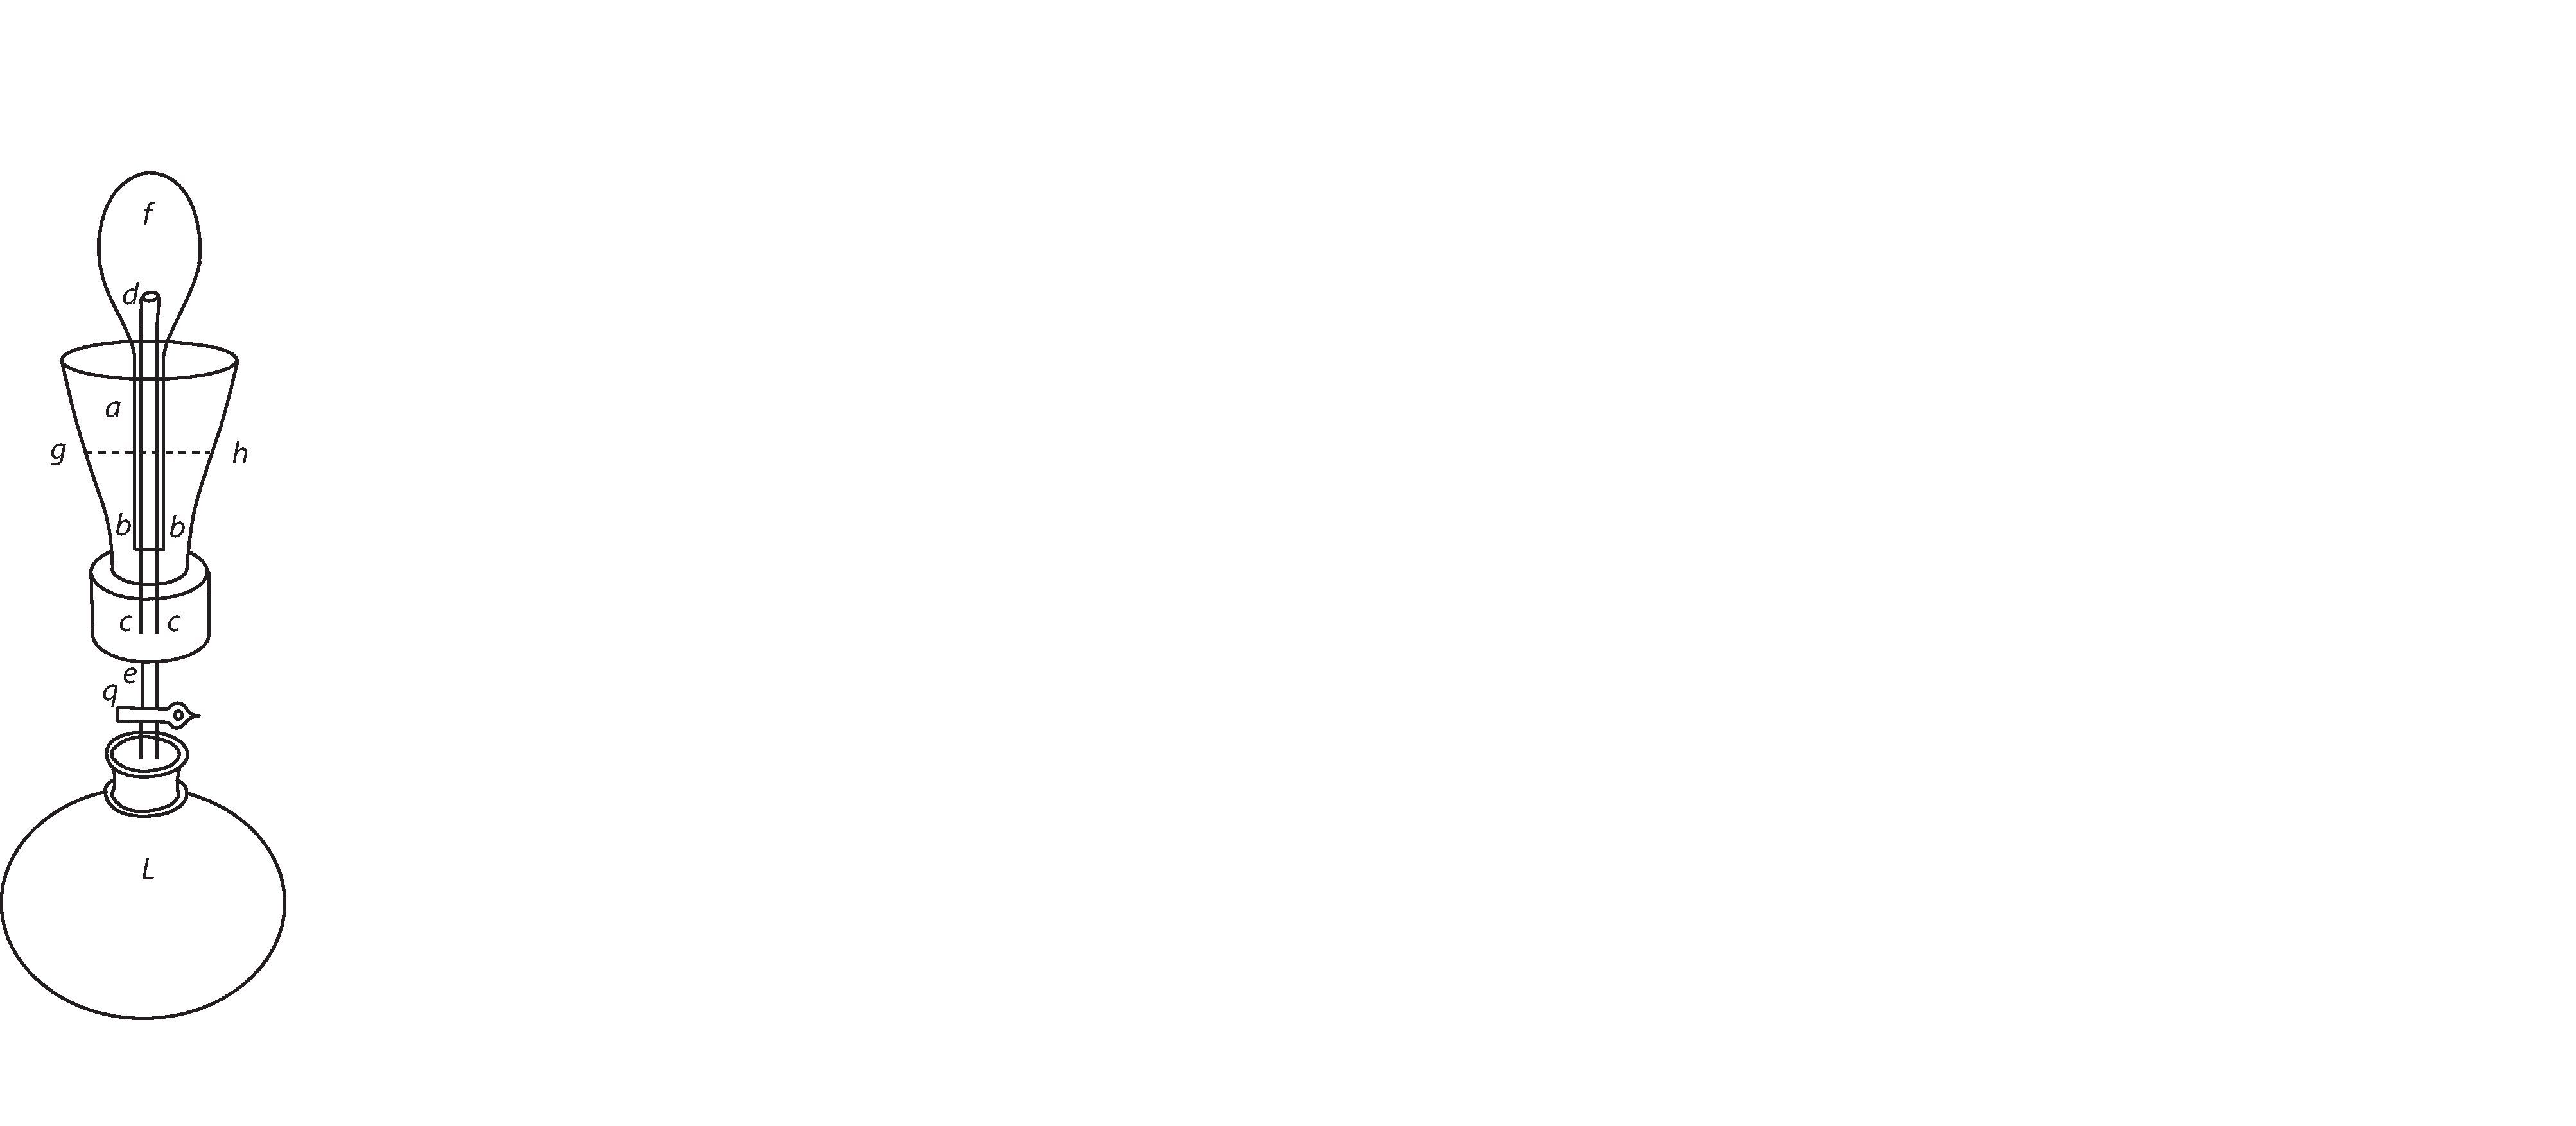
\includegraphics[width=0.24\textwidth]{images/LH35_14_2_94r1}\\\textit{[Fig. 3]} 
                        %\caption{Bildbeschreibung}
                      \end{center}